\textbf{Swagger UI} - это инструмент для визуализации и тестирования RESTful API,
который позволяет легко и удобно отображать документацию API в интерактивном формате.
Swagger UI позволяет пользователям легко узнать, как использовать API, просматривать доступные методы и параметры, а также тестировать их напрямую из интерфейса.

NestJS предоставляет мощный интегрированный инструмент для создания и документирования API - Swagger Module.
Этот модуль автоматически генерирует документацию API на основе встроенных декораторов и аннотаций,
что делает процесс создания документации проще и быстрее.
Кроме того, Swagger Module позволяет легко интегрировать Swagger UI в приложение,
чтобы пользователи могли удобно просматривать и тестировать API.

При использовании NestJS и Swagger Module, можено значительно сократить время и усилия,
затрачиваемые на создание и документирование API.
NestJS обеспечивает простоту и гибкость при создании API, а Swagger Module делает процесс документирования быстрым и удобным.
Кроме того, Swagger UI предоставляет простой и понятный интерфейс для тестирования API,
что делает процесс отладки более эффективным. Все это делает NestJS лучшим выбором для создания и документирования API,
особенно если хотим сэкономить время и усилия при разработке.

\textbf{Эндпоинт} (англ. endpoint) - это конечная точка (адрес) веб-сервера, доступная для запросов от клиентского приложения.
В контексте веб-разработки эндпоинт обычно является частью RESTful API (Representational State Transfer API)
и представляет собой конечную точку, к которой можно отправить запросы для выполнения определенного действия или получения определенной информации.

Например, если мы хотим получить информацию о товаре с определенным идентификатором,
мы можем отправить запрос на эндпоинт веб-сервера, который обрабатывает такие запросы и возвращает запрашиваемую информацию в определенном формате,
например, JSON или XML.

Эндпоинт может обрабатывать различные типы запросов, такие как GET, POST, PATCH, PUT или DELETE,
в зависимости от того, какие действия должны быть выполнены с данными на сервере.
Кроме того, эндпоинт может быть защищен авторизацией, чтобы предотвратить несанкционированный доступ к конфиденциальным данным или функциональности.

\textbf{Эндпоинт <<users>>} связан с управлением учётными записями пользователей.
Благодаря данному эндпоинту, пользователи имеют возможность выполнять следующие операции:
регистрацию новой учётной записи,
активацию аккаунта,
запрос на смену электронной почты,
подтверждение смены адреса электронной почты,
отмену запроса на смену адреса электронной почты,
восстановление забытого пароля,
а также изменение пароля текущей учётной записи.

Эндпоинт <<users>> представлен на рис.~\ref{fig:swagger_users}.

\begin{figure}[!p]
    \centering

    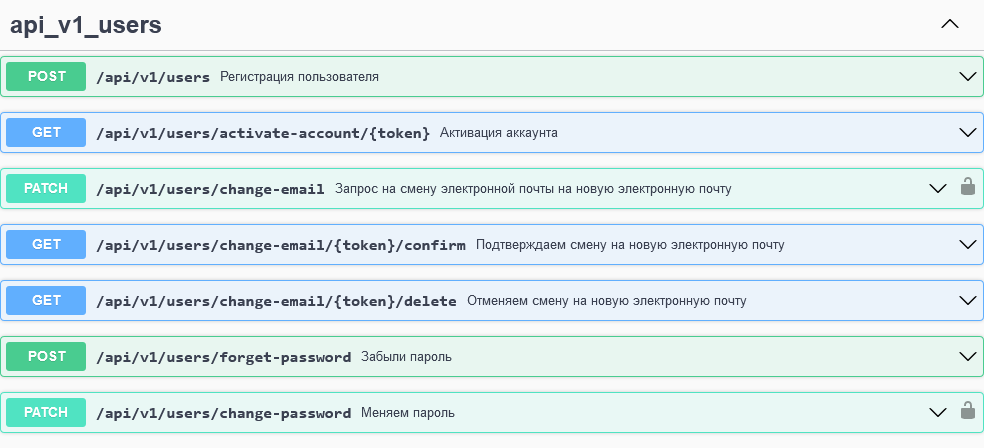
\includegraphics[width=12cm]
    {images/swagger/users.png}

    \caption{Эндпоинт <<users>>}

    \label{fig:swagger_users}
\end{figure}

\textbf{Эндпоинт <<sessions>>} в приложении играет важную роль,
предоставляя возможность пользователям войти в свой аккаунт и получить доступ к различным функциям.
С помощью этого эндпоинта можно получить доступ к списку активных сессий,
обновить существующую сессию для получения нового токенов доступа.
Также эндпоинт <<sessions>> позволяет закрыть текущую сессию или все активные сессии,
что обеспечивает безопасность аккаунта пользователя.
В целом, этот эндпоинт является важным инструментом для управления сессиями пользователей и обеспечения безопасности данных в приложении.

Эндпоинт <<sessions>> представлен на рис.~\ref{fig:swagger_sessions}.

\begin{figure}[!p]
    \centering

    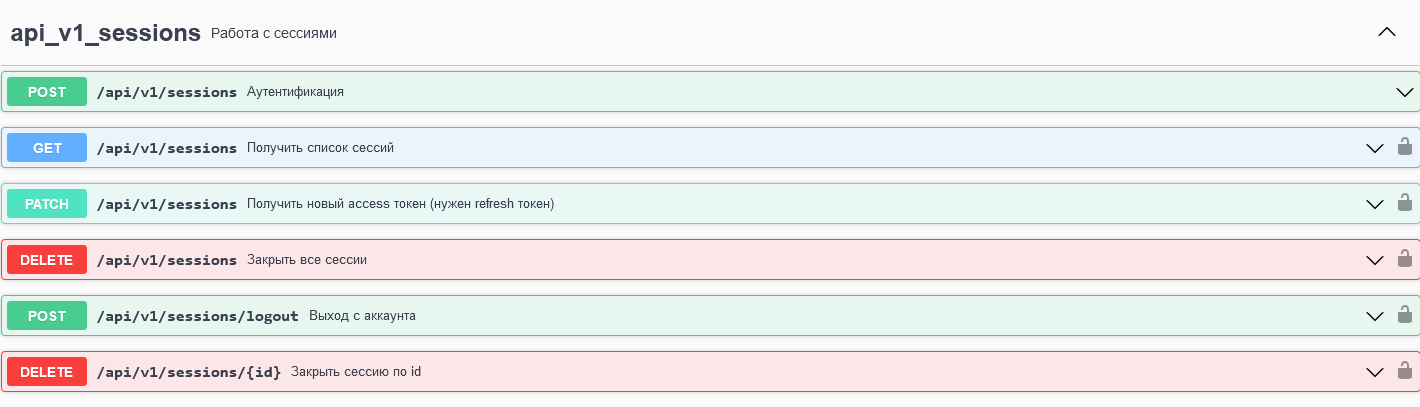
\includegraphics[width=12cm]
    {images/swagger/sessions.png}

    \caption{Эндпоинт <<sessions>>}

    \label{fig:swagger_sessions}
\end{figure}

\textbf{Эндпоинт item-brands} предназначен для осуществления операций CRUD (Create, Read, Update, Delete) с производителями номенклатуры.
Здесь вы можете создавать новых производителей, просматривать информацию о них, обновлять данные и удалять производителей, если это необходимо

Эндпоинт <<item-brands>> представлен на рис.~\ref{fig:swagger_item_brands}.

\begin{figure}[!p]
    \centering

    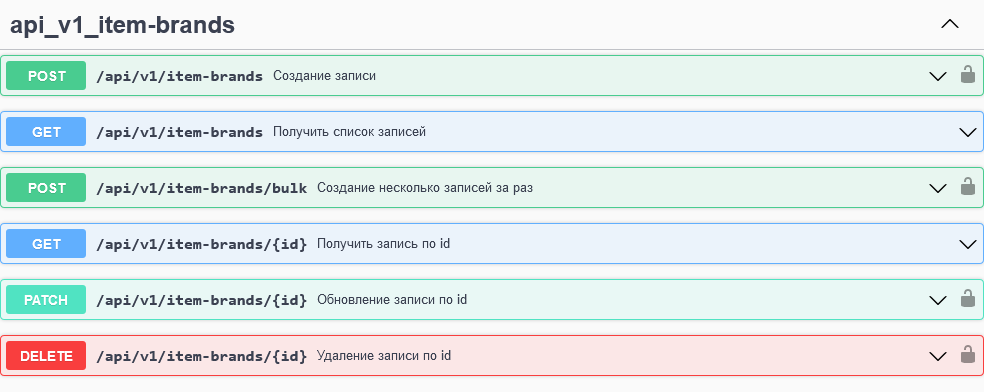
\includegraphics[width=12cm]
    {images/swagger/item-brands.png}

    \caption{Эндпоинт <<item-brands>>}

    \label{fig:swagger_item_brands}
\end{figure}

\textbf{Эндпоинт item-categories} предназначен для управления категориями номенклатуры,
включающего в себя операции CRUD (Create, Read, Update, Delete).
Здесь вы сможете создавать, просматривать, обновлять и удалять категории, а также получать информацию о них.

Эндпоинт <<item-brands>> представлен на рис.~\ref{fig:swagger_item_categories}.

\begin{figure}[!p]
    \centering

    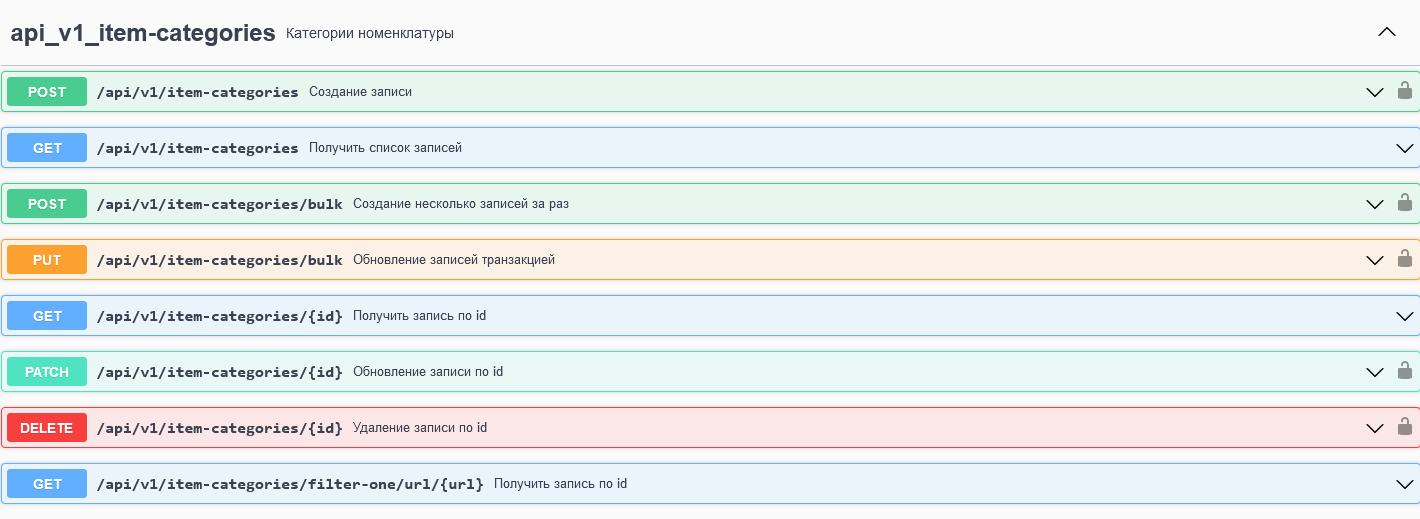
\includegraphics[width=12cm]
    {images/swagger/item-categories.png}

    \caption{Эндпоинт <<item-categories>>}

    \label{fig:swagger_item_categories}
\end{figure}

\textbf{Эндпоинт <<item-characteristics>>} обеспечивает набор CRUD-операций для типов характеристик номенклатуры.

Эндпоинт <<item-characteristics>> представлен на рис.~\ref{fig:swagger_item_characteristics}.

\begin{figure}[!p]
    \centering

    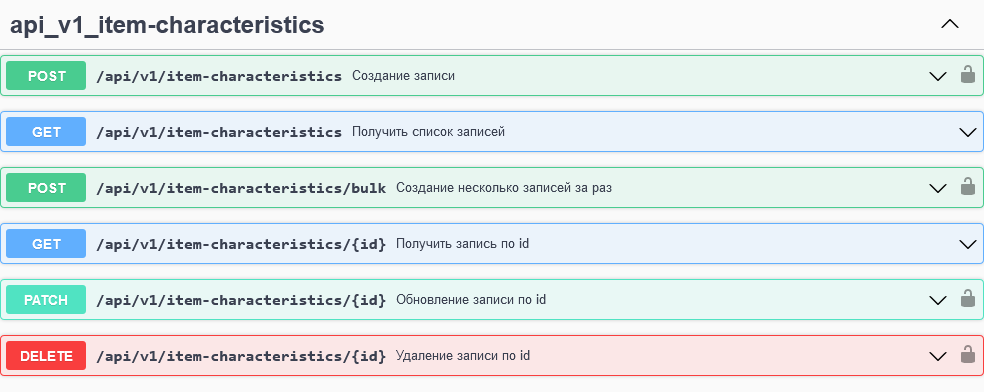
\includegraphics[width=16cm]
    {images/swagger/item-characteristics.png}

    \caption{Эндпоинт <<item-characteristics>>}

    \label{fig:swagger_item_characteristics}
\end{figure}

\textbf{Эндпоинт <<items>>} представляет набор операций CRUD для управления номенклатурой.
Кроме того, он позволяет добавлять и редактировать табличные части, включая список характеристик номенклатуры и ссылок на картинки.
Это дает возможность удобно и эффективно управлять всей информацией, связанной с конкретной номенклатурой в едином месте.

Эндпоинт <<items>> представлен на рис.~\ref{fig:swagger_items}.

\begin{figure}[!p]
    \centering

    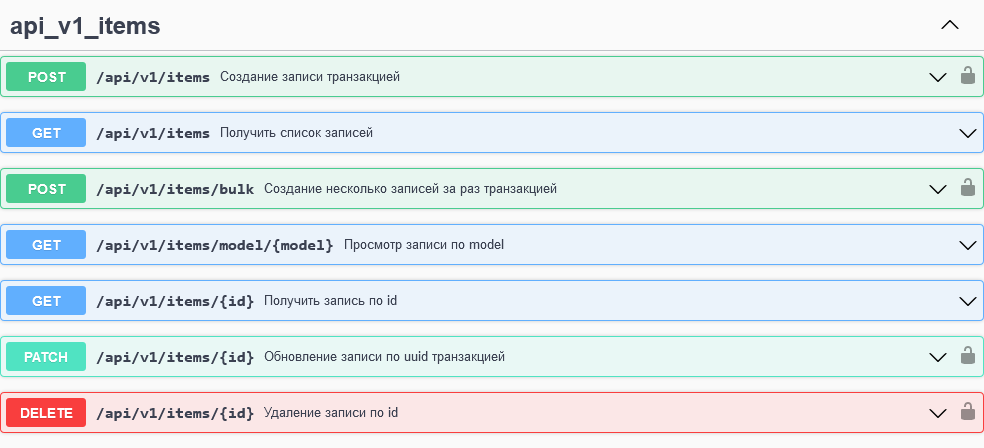
\includegraphics[width=16cm]
    {images/swagger/items.png}

    \caption{Эндпоинт <<items>>}

    \label{fig:swagger_items}
\end{figure}

\textbf{Эндпоинт <<articles>>} предоставляет возможность выполнения операций CRUD (Create, Read, Update, Delete) для управления статьями в приложении,
такими как новости или блог.
С помощью этого эндпоинта можно создавать, читать, обновлять и удалять статьи,
а также получать список всех статей или выборочно по фильтру.

Эндпоинт <<articles>> представлен на рис.~\ref{fig:swagger_articles}.

\begin{figure}[!p]
    \centering

    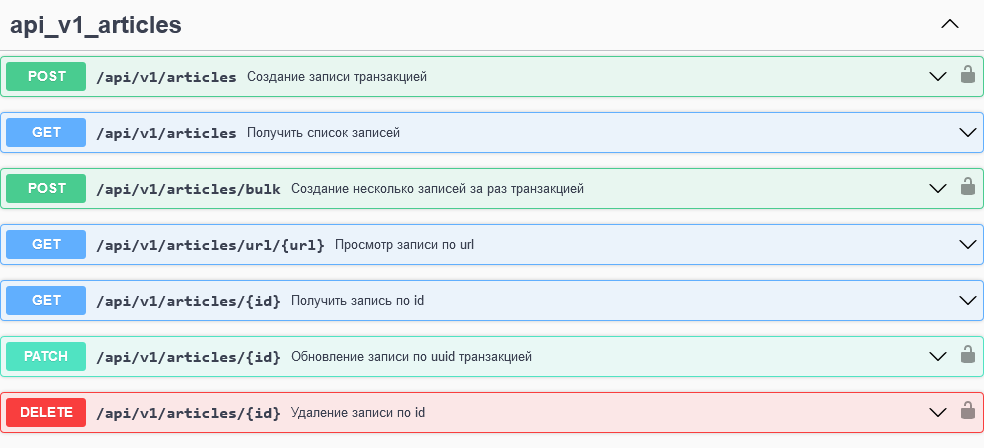
\includegraphics[width=16cm]
    {images/swagger/articles.png}

    \caption{Эндпоинт <<articles>>}

    \label{fig:swagger_articles}
\end{figure}

\textbf{Эндпоинт <<contact-types>>} представляет собой CRUD-интерфейс для управления типами контактов,
таких как email, phone, viber, whatsapp, telegram, skype.
Они являются ключевыми элементами для связи многих к одному и многих ко многим.

Эндпоинт <<contact-types>> представлен на рис.~\ref{fig:swagger_contact_types}.

\begin{figure}[!p]
    \centering

    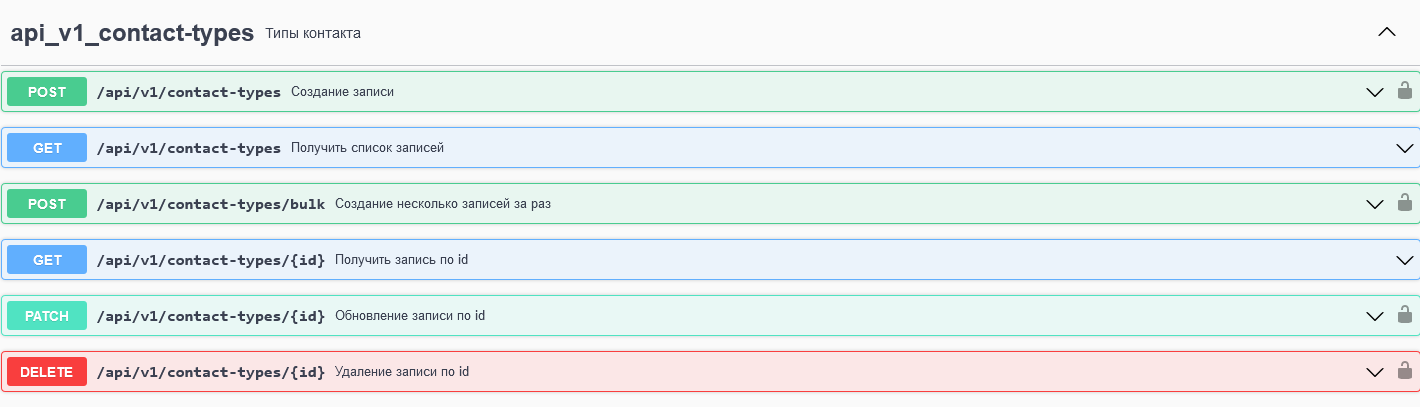
\includegraphics[width=16cm]
    {images/swagger/contact-types.png}

    \caption{Эндпоинт <<contact-types>>}

    \label{fig:swagger_contact_types}
\end{figure}

\textbf{Эндпоинт <<helpers>>} представляет полноценный CRUD-интерфейс для создания и управления контактами,
которые помогают клиентам быстро и легко связаться с компанией.
Этот эндпоинт также включает в себя удобную табличную часть,
которая позволяет добавлять и редактировать различные типы контактов,
такие как email, phone, viber, whatsapp, telegram, skype, для удобства клиентов.

Эндпоинт <<helpers>> представлен на рис.~\ref{fig:swagger_helpers}.

\begin{figure}[!p]
    \centering

    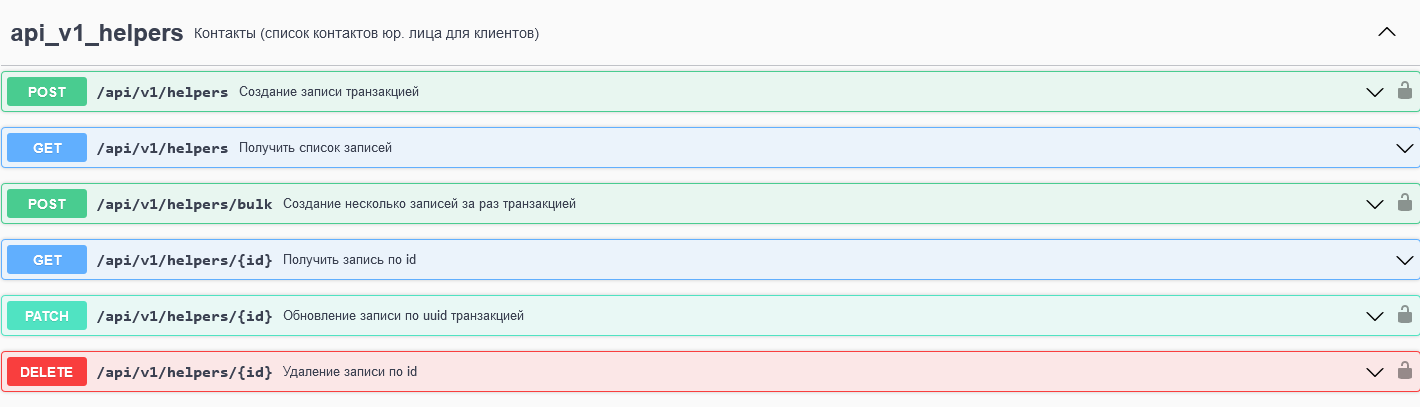
\includegraphics[width=16cm]
    {images/swagger/helpers.png}

    \caption{Эндпоинт <<helpers>>}

    \label{fig:swagger_helpers}
\end{figure}

\textbf{Эндпоинт <<orders>>} представляет собой важный механизм оформления заказов.
Он позволяет пользователям отправлять заявки на приобретение товаров,
которые затем записываются в базу данных.
Кроме того, эндпоинт позволяет отменять заказы и помечать их как закрытые модераторами, когда номенклатура уже доставлена. 

Эндпоинт <<orders>> представлен на рис.~\ref{fig:swagger_orders}.

\begin{sidewaystable}
    \small
    \caption{Повернутая таблица} \label{tabl:swagger}

    \begin{tabular}{|p{1cm}|p{1cm}|p{8.5cm}|p{4.8cm}|p{8.5cm}|}
        \hline
        \multicolumn{1}{|c|}{Роль}
        & \multicolumn{1}{c|}{Метод}
        & \multicolumn{1}{c|}{Эндпоинт}
        & \multicolumn{1}{c|}{Коды}
        & \multicolumn{1}{c|}{Назначение}
        \\ \hline

        any & post & /api/v1/users & 200, 409, 500 & регистрация \\ \hline 
        admin & get & /api/v1/users & 200, 401, 404, 500 & получение списка пользователей \\ \hline 
        any & get & /api/v1/users/activate-account/\{token\} & 200, 404, 500 & активация аккаунта \\ \hline 
        user & patch & /api/v1/users/change-email & 200, 401, 409, 429, 500 & запрос на смену email \\ \hline 
        any & get & /api/v1/users/change-email/\{token\}/confirm & 200, 404, 500 & подтверждение смены email \\ \hline 
        any & get & /api/v1/users/change-email/\{token\}/delete & 200, 404, 500 & отмена смены email \\ \hline 
        any & post & /api/v1/users/forget-password & 200, 409, 500 & запросить логин и новый пароль \\ \hline 
        user & patch & /api/v1/users/change-password & 200, 401, 409, 500 & смена пароля \\ \hline
        admin & post & /api/v1/users/is-admin & 200, 401, 500 & проверка роли администратора\\ \hline 
        any & post & /api/v1/sessions & 201, 409, 500 & вход в аккаунт \\ \hline 
        user & get & /api/v1/sessions & 200, 401, 500 & получаем список сессий \\ \hline 
        any & patch & /api/v1/sessions & 200, 401, 500 & обновление токена доступа \\ \hline 
        user & delete & /api/v1/sessions & 200, 401, 500 & закрытие всех сессий \\ \hline 
        user & post & /api/v1/sessions/logout & 200, 500 & выход с аккаунта \\ \hline 
        user & delete & /api/v1/sessions/\{id\} & 200, 401, 500 & закрытие сессий по id \\ \hline 
        any & get & /api/v1/apk-versions & 200, 500 & получить последнию версию apk \\ \hline 
        admin & post & /api/v1/item-characteristics & 201, 400, 401, 409, 500 & создание характеристики \\ \hline 
        any & get & /api/v1/item-characteristics & 200, 500 & просмотр списка характеристик \\ \hline 
        admin & post & /api/v1/item-characteristics/bulk & 201, 400, 401, 409, 500 & добавление несколько характеристик за раз \\ \hline 
        admin & put & /api/v1/item-characteristics/bulk & 200, 400, 401, 409, 500 & обновление несколько характеристик за раз \\ \hline 
        any & get & /api/v1/item-characteristics/\{id\} & 200, 404, 500 & просмотр характеристики по id \\ \hline 
        admin & patch & /api/v1/item-characteristics/\{id\} & 200, 400, 401, 404, 409, 500 & обновление характеристики по id \\ \hline 
        admin & delete & /api/v1/item-characteristics/\{id\} & 200, 401, 404, 500 & удаление характеристики по id \\ \hline 
        admin & post & /api/v1/item-brands & 201, 400, 401, 409, 500 & создание бренда \\ \hline 
        any & get & /api/v1/item-brands & 200, 500 & получение спика брендов \\ \hline  
        \multicolumn{5}{l}{Продолжение таблицы~\ref{tabl:swagger} на следующей странице} \\
    \end{tabular}
\end{sidewaystable}
\begin{sidewaystable}
    \small
    % \caption{Повернутая таблица}

    \begin{tabular}{|p{1cm}|p{1cm}|p{8.5cm}|p{4.8cm}|p{8.5cm}|}
        \multicolumn{5}{c}{Продолжение таблицы~\ref{tabl:swagger}} \\
        \hline
        \multicolumn{1}{|c|}{Роль}
        & \multicolumn{1}{c|}{Метод}
        & \multicolumn{1}{c|}{Эндпоинт}
        & \multicolumn{1}{c|}{Коды}
        & \multicolumn{1}{c|}{Назначение}
        \\ \hline
        admin & post & /api/v1/item-brands/bulk & 201, 400, 401, 409, 500 & создание несколько брендов за раз \\ \hline 
        admin & put & /api/v1/item-brands/bulk & 200, 400, 401, 404, 409, 500 & обновление несколько бренда за раз \\ \hline
        any & get & /api/v1/item-brands/\{id\} & 200, 404, 500 & просмотр бренда по id \\ \hline 
        admin & patch & /api/v1/item-brands/\{id\} & 200, 400, 401, 409, 500 & обновление бренда по id \\ \hline 
        admin & delete & /api/v1/item-brands/\{id\} & 200, 401, 404, 500 & удаление бренда по id \\ \hline 
        any & delete & /api/v1/item-brands/filter-one/url/\{url\} & 200, 404, 500 & получение бренда по url \\ \hline 
        admin & post & /api/v1/item-categories & 201, 400, 401, 409, 500 & создание категории \\ \hline 
        any & get & /api/v1/item-categories & 200, 500 & просмотр списка категорий \\ \hline 
        admin & post & /api/v1/item-categories/bulk & 201, 400, 401, 409, 500 & создание несколько категорий за раз \\ \hline 
        admin & put & /api/v1/item-categories/bulk & 200, 400, 401, 400, 409, 500 & обновление несколько категорий за раз \\ \hline 
        any & get & /api/v1/item-categories/\{id\} & 200, 404, 500 & просмотр категории по id \\ \hline 
        admin & patch & /api/v1/item-categories/\{id\} & 200, 400, 401, 404, 409, 500 & обновление категории по id \\ \hline 
        admin & delete & /api/v1/item-categories/\{id\} & 200, 401, 404, 500 & удаление категории по id \\ \hline 
        any & delete & /api/v1/item-categories/filter-one/\{url\} & 200, 404, 500 & получение категори по url \\ \hline 
        admin & post & /api/v1/items & 201, 400, 401, 409, 500 & создание товара \\ \hline 
        any & get & /api/v1/items & 200, 500 & получение списка товаров \\ \hline 
        admin & post & /api/v1/items/bulk & 201, 400, 401, 409, 500 & создание несколько товаров за раз \\ \hline 
        admin & put & /api/v1/items/bulk & 200, 400, 401, 404, 409, 500 & обновление несколько товаров за раз \\ \hline 
        any & get & /api/v1/items/filter-one/model/\{model\} & 200, 404, 500 & получение товара по модели \\ \hline 
        any & post & /api/v1/items/filter/models & 200, 500 & получение списка товаров по списку моделей \\ \hline
        any & post & /api/v1/items/filter/ids & 200, 500 & получение списка товаров по списку id \\ \hline  
        any & get & /api/v1/items/search/\{search\} & 200, 500 & получение 5 штук товаров по поиску \\ \hline 
        any & get & /api/v1/items/search-all/\{search\} & 200, 500 & получение всех товаров подходящие поиску \\ \hline 
        any & get & /api/v1/items/\{id\} & 200, 404, 500 & получение товара по id \\ \hline 
        admin & patch & /api/v1/items/\{id\} & 200, 400, 401, 404, 409, 500 & обновление товара по id \\ \hline 
        admin & delete & /api/v1/items/\{id\} & 200, 401, 404, 500 & удаление товара по id \\ \hline 
        \multicolumn{5}{l}{Продолжение таблицы~\ref{tabl:swagger} на следующей странице}
    \end{tabular}
\end{sidewaystable}
\begin{sidewaystable}
    \small
    % \caption{Повернутая таблица}
    \begin{tabular}{|p{1cm}|p{1cm}|p{8.5cm}|p{4.8cm}|p{8.5cm}|}
        \multicolumn{5}{c}{Продолжение таблицы~\ref{tabl:swagger}} \\
        \hline
        \multicolumn{1}{|c|}{Роль}
        & \multicolumn{1}{c|}{Метод}
        & \multicolumn{1}{c|}{Эндпоинт}
        & \multicolumn{1}{c|}{Коды}
        & \multicolumn{1}{c|}{Назначение}
        \\ \hline
        user & post & /api/v1/favorite-items/\{itemId\} & 201, 401, 500 & добавление товара в избранные \\ \hline 
        user & delete & /api/v1/favorite-items/\{itemId\} & 200, 401, 404, 500 & удаление товара из избранных \\ \hline 
        user & get & /api/v1/favorite-items & 200, 500 & получение списка избранных \\ \hline 
        user & post & /api/v1/order & 201 & создание заявки \\ \hline 
        any & get & /api/v1/order & 200 & получение списка заявок \\ \hline 
        user & get & /api/v1/order/\{id\} & 200 & получение заявки по id \\ \hline 
        moder & patch & /api/v1/order/\{id\}/completed & 200 & заявка выполнена \\ \hline 
        user & patch & /api/v1/order/\{id\}/cancel & 200 & отменить заявку \\ \hline 
        admin & post & /api/v1/articles & 201, 400, 401 & создание новости \\ \hline 
        any & get & /api/v1/articles & 200, 500 & получение списка новостей \\ \hline 
        admin & post & /api/v1/articles/bulk & 201, 400, 401, 409, 500 & создание несколько новостей за раз \\ \hline 
        any & get & /api/v1/articles/filter-one/url/\{url\} & 200, 404, 500 & получение новости по ur; \\ \hline 
        any & get & /api/v1/articles/\{id\} & 200, 404, 500 & получение новости по id \\ \hline 
        admin & patch & /api/v1/articles/\{id\} & 200, 400 401, 404, 409, 500 & обновление новости по id \\ \hline 
        admin & delete & /api/v1/articles/\{id\} & 200, 401, 404, 500 & удаление новости по id \\ \hline  
        admin & post & /api/v1/contact-types & 201, 400, 401, 409, 500 & создание типа контакта \\ \hline 
        any & get & /api/v1/contact-types & 200, 500 & просмотр списка типов контактов \\ \hline 
        admin & post & /api/v1/contact-types/bulk & 201, 400, 401, 409, 500 & создание несколько типов контактов \\ \hline 
        any & get & /api/v1/contact-types/\{id\} & 200, 404, 500 & просмотр типа контакта по id \\ \hline 
        admin & patch & /api/v1/contact-types/\{id\} & 200, 400, 401, 404, 409, 500 & обновление типа контакта по id \\ \hline 
        admin & delete & /api/v1/contact-types/\{id\} & 200, 401, 404, 500 & удаление типа контакта по id \\ \hline 
        admin & post & /api/v1/helpers & 201, 400, 401, 500 & создание помощника \\ \hline 
        any & get & /api/v1/helpers & 200, 500 & получение списка помощников \\ \hline 
        admin & post & /api/v1/helpers/bulk & 201, 400, 401, 500 & создание несколько помощников за раз \\ \hline 
        any & get & /api/v1/helpers/\{id\} & 200, 404, 500 & просмотр помощника по id \\ \hline 
        admin & patch & /api/v1/helpers/\{id\} & 200, 400, 401, 404, 500 & обновление помощника по id \\ \hline 
        admin & delete & /api/v1/helpers/\{id\} & 200, 401, 404, 500 & удаление помощника по id \\ \hline 
    \end{tabular}
\end{sidewaystable}

\textbf{Экраны с номенклатурой} на Android изображены на рис.~\ref{fig:android_items}.
\textbf{Экраны со статьями} на Android изображены на рис.~\ref{fig:android_articles}.
\textbf{Экраны с корзиной и указанием количества} изображены на рис.~\ref{fig:android_basket}.
\textbf{Экраны с входом в аккаунт, восстановлением пароля и проверки обновления} изображены на рис.~\ref{fig:android_login}.
\textbf{Экраны с регистрацией юридического лица} изображены на рис.~\ref{fig:android_registration}.

\begin{figure}[!p]
    \centering

    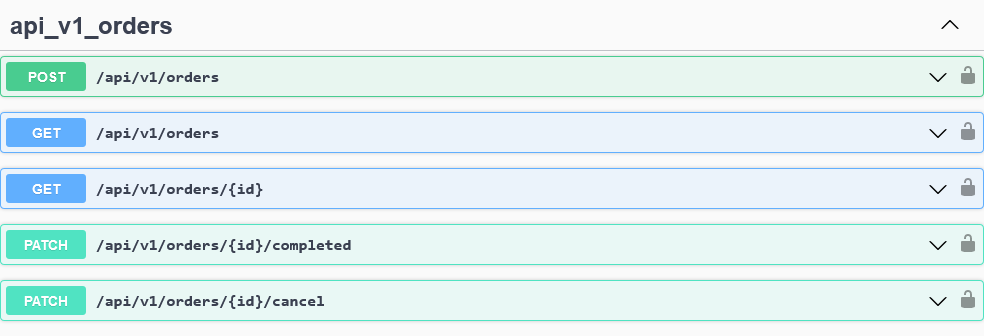
\includegraphics[width=16cm]
    {images/swagger/orders.png}

    \caption{Эндпоинт <<orders>>}

    \label{fig:swagger_orders}
\end{figure}

\begin{figure}[!p]\centering
    \begin{minipage}{0.24\textwidth}
        \centering

        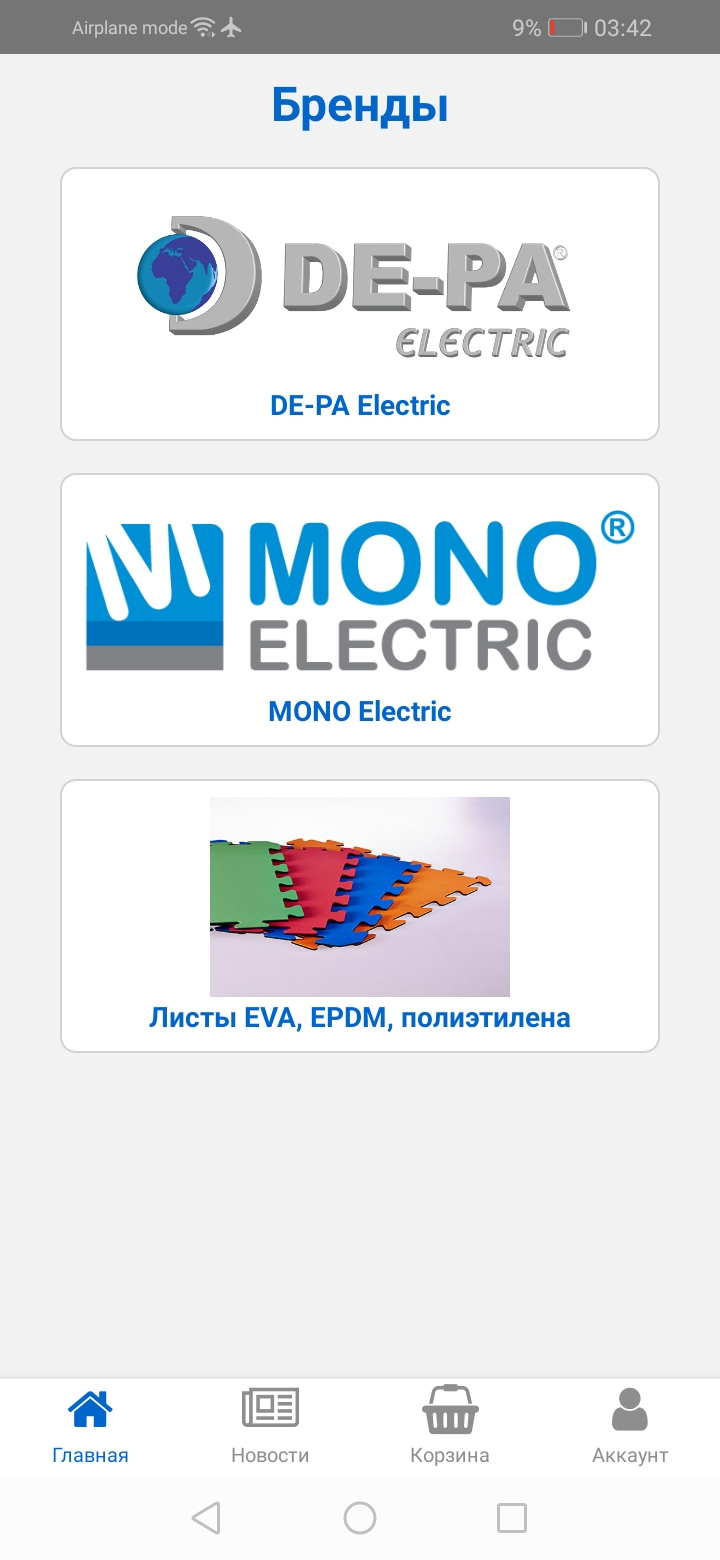
\includegraphics[height=7cm]
        {images/android/item-brands.jpg}
    \end{minipage}
    \begin{minipage}{0.24\textwidth}
        \centering

        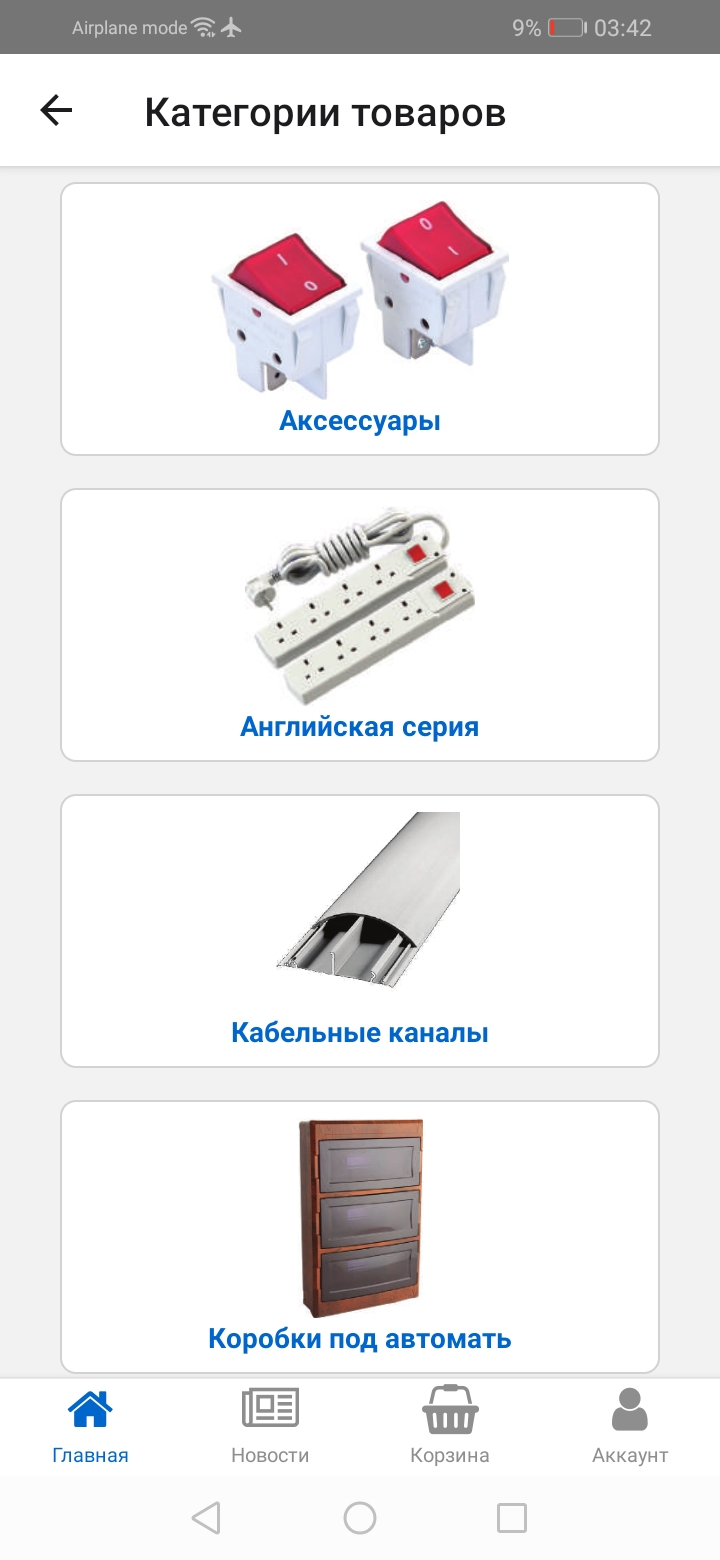
\includegraphics[height=7cm]
        {images/android/item-categories.jpg}
    \end{minipage}
    \begin{minipage}{0.24\textwidth}
        \centering

        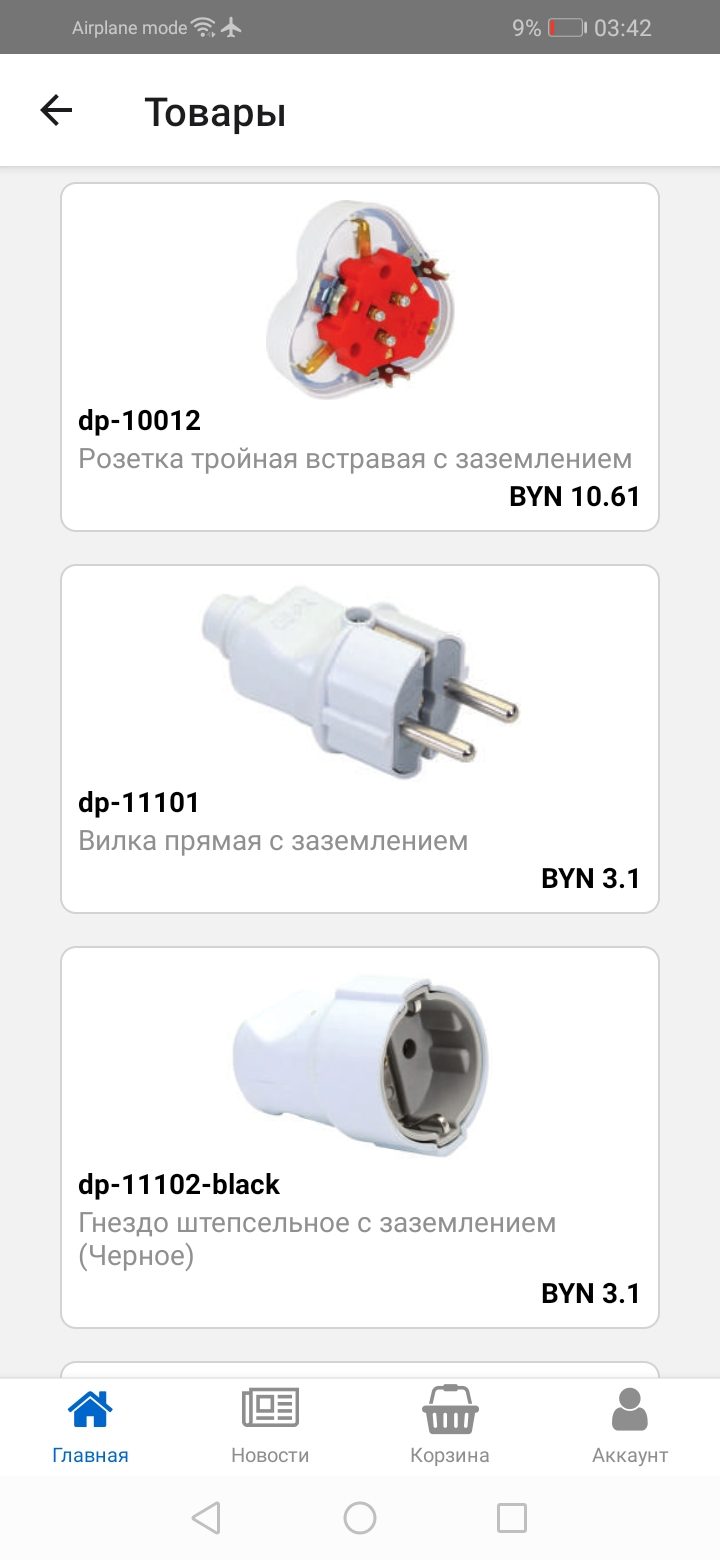
\includegraphics[height=7cm]
        {images/android/items.jpg}
    \end{minipage}
    \begin{minipage}{0.24\textwidth}
        \centering

        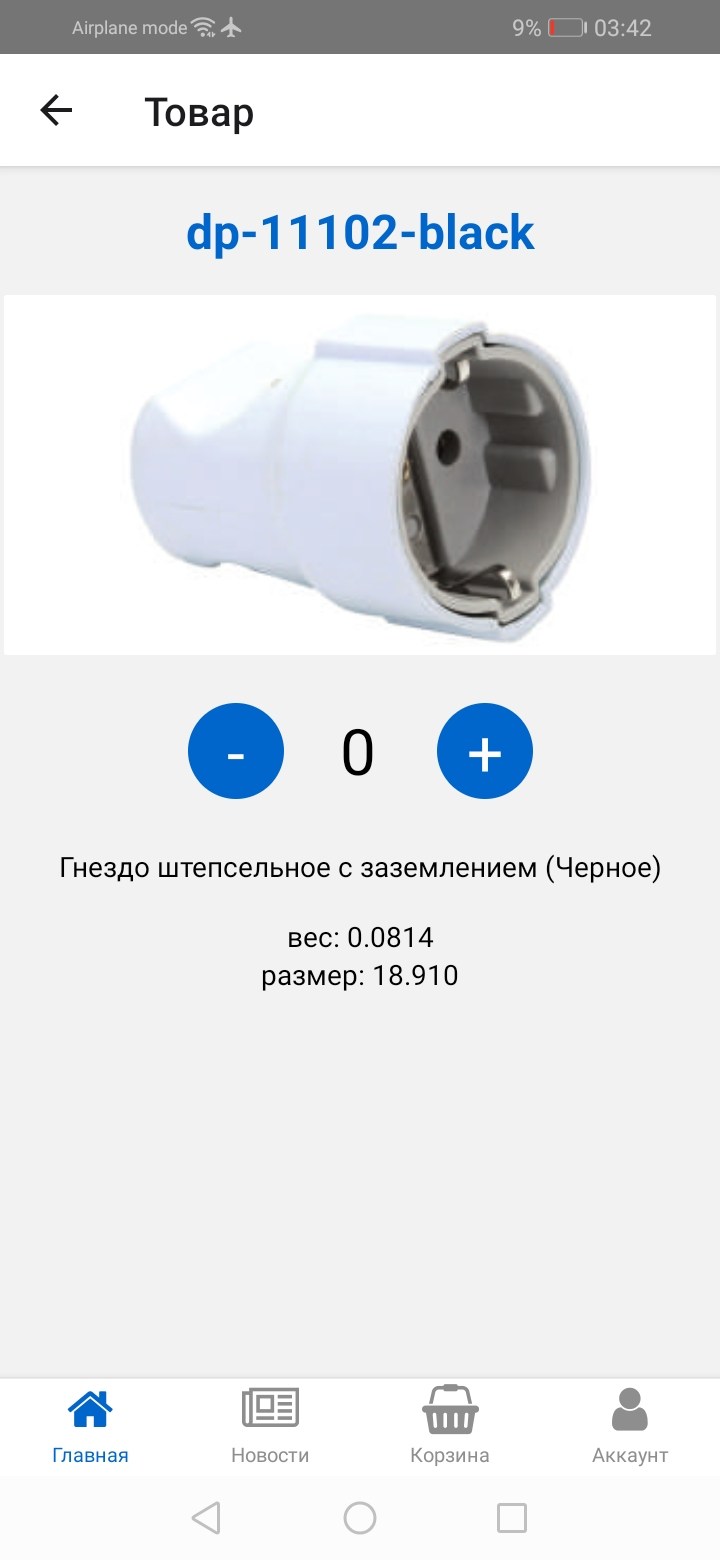
\includegraphics[height=7cm]
        {images/android/item.jpg}
    \end{minipage}

    \caption{Производители, категории, товары и сам товар}
    \label{fig:android_items}
\end{figure}

\begin{figure}[!p]\centering
    \begin{minipage}{0.19\textwidth}
        \centering

        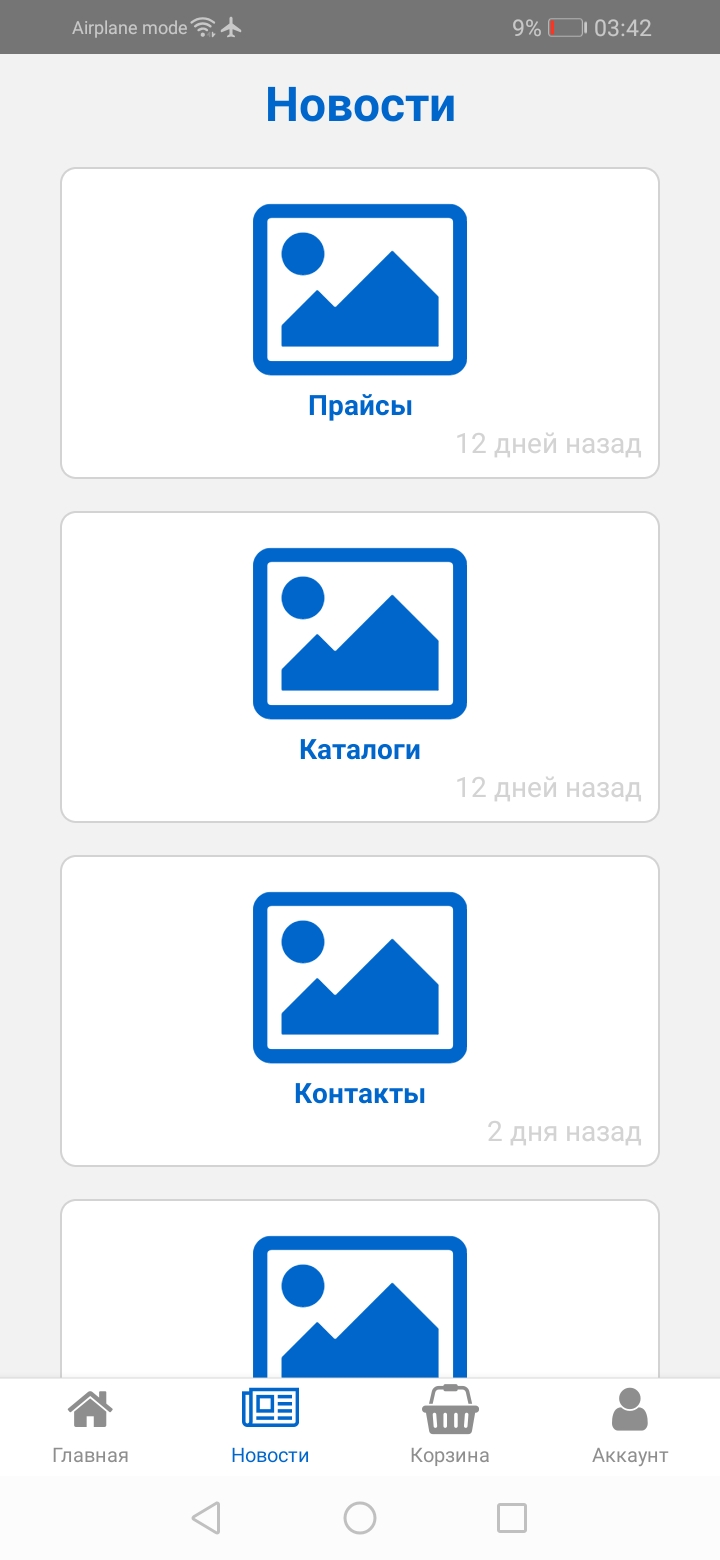
\includegraphics[width=.99\linewidth]
        {images/android/articles.jpg}
    \end{minipage}
    \begin{minipage}{0.19\textwidth}
        \centering

        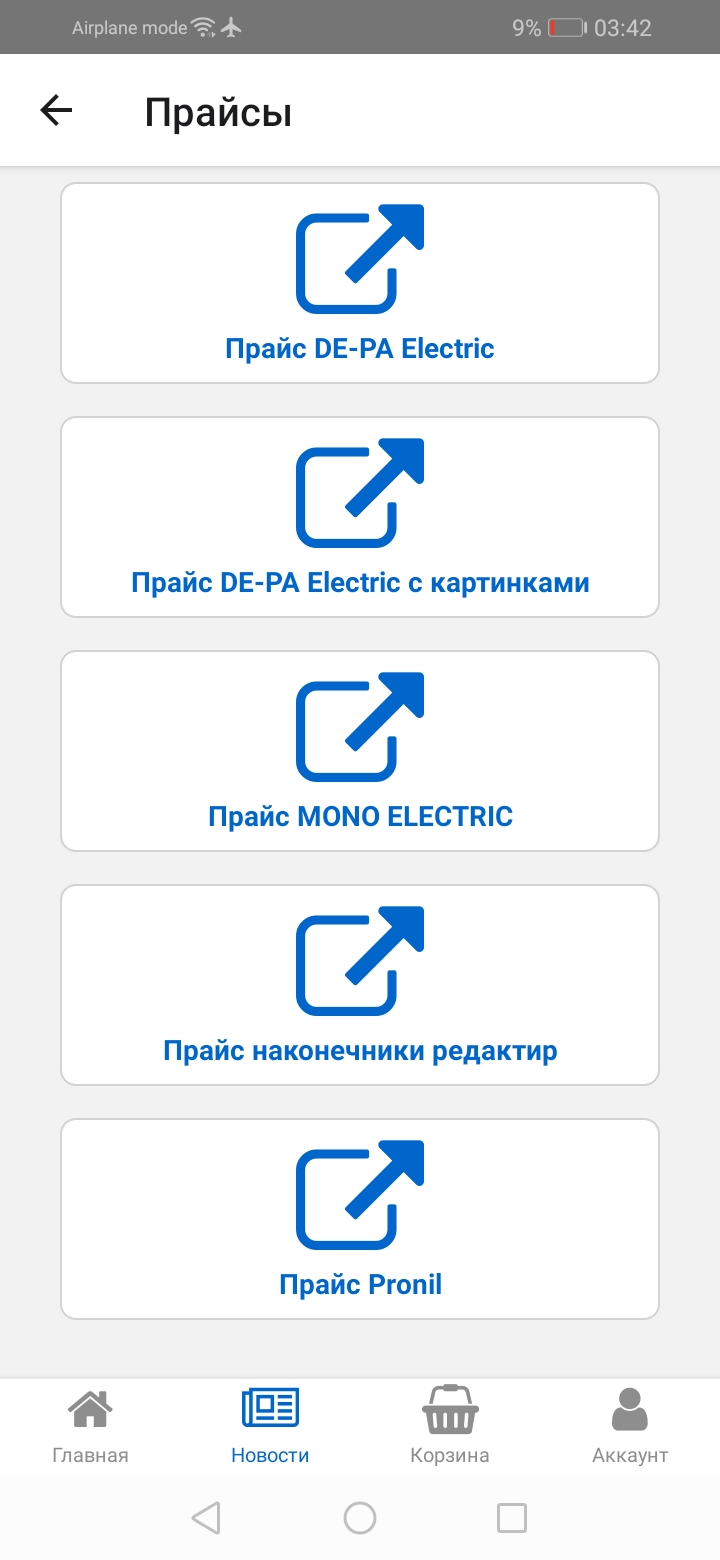
\includegraphics[width=.99\linewidth]
        {images/android/article-prices.jpg}
    \end{minipage}
    \begin{minipage}{0.19\textwidth}
        \centering

        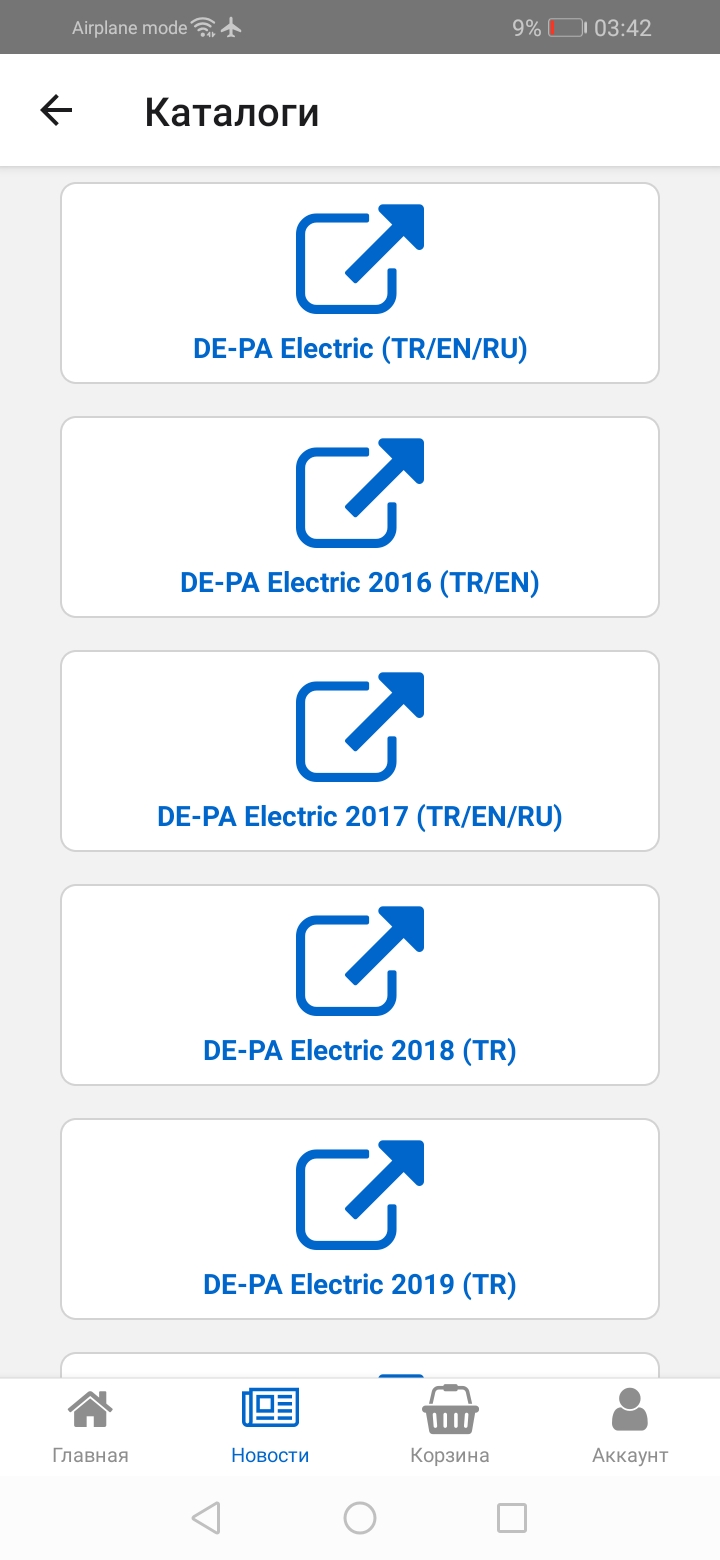
\includegraphics[width=.99\linewidth]
        {images/android/article-catalogs.jpg}
    \end{minipage}
    \begin{minipage}{0.19\textwidth}
        \centering

        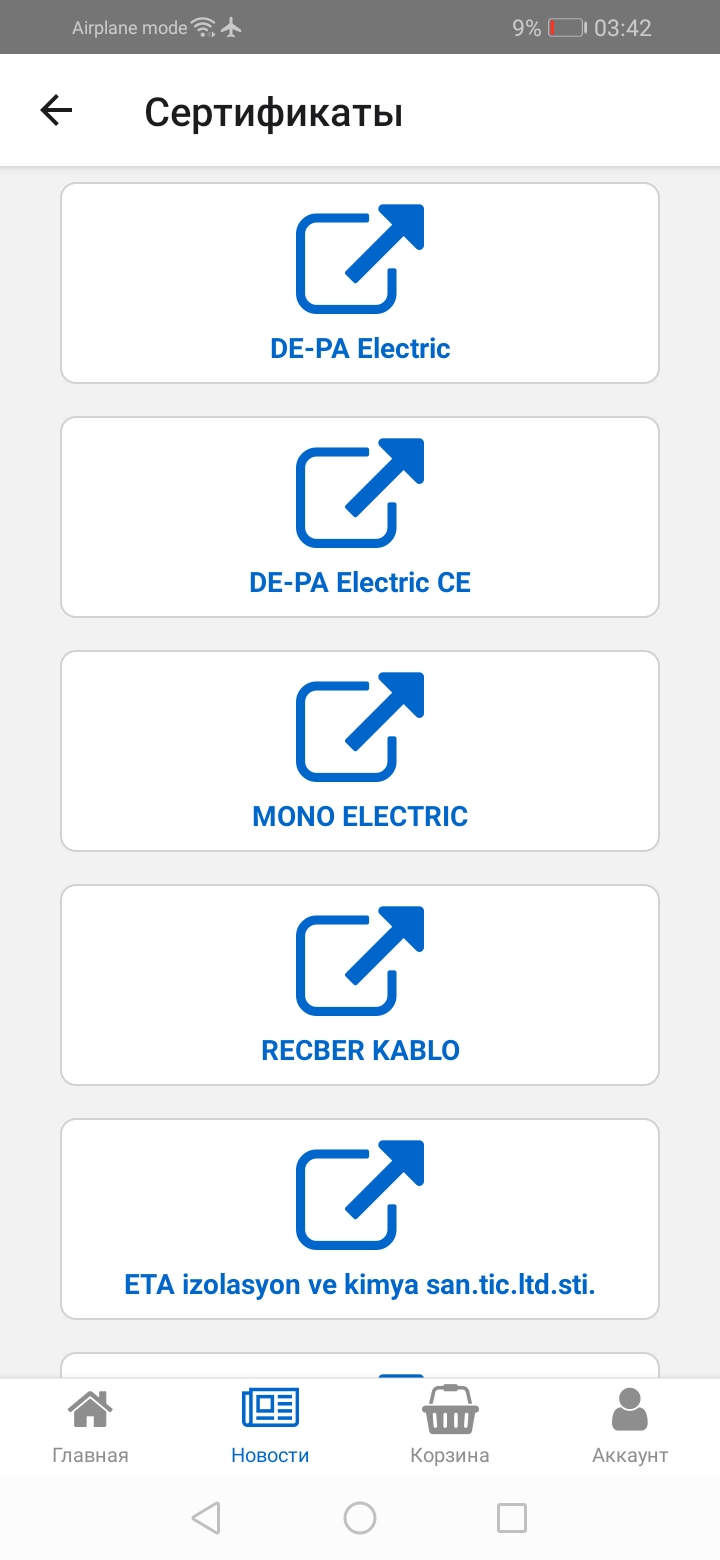
\includegraphics[width=.99\linewidth]
        {images/android/article-certificates.jpg}
    \end{minipage}
    \begin{minipage}{0.19\textwidth}
        \centering

        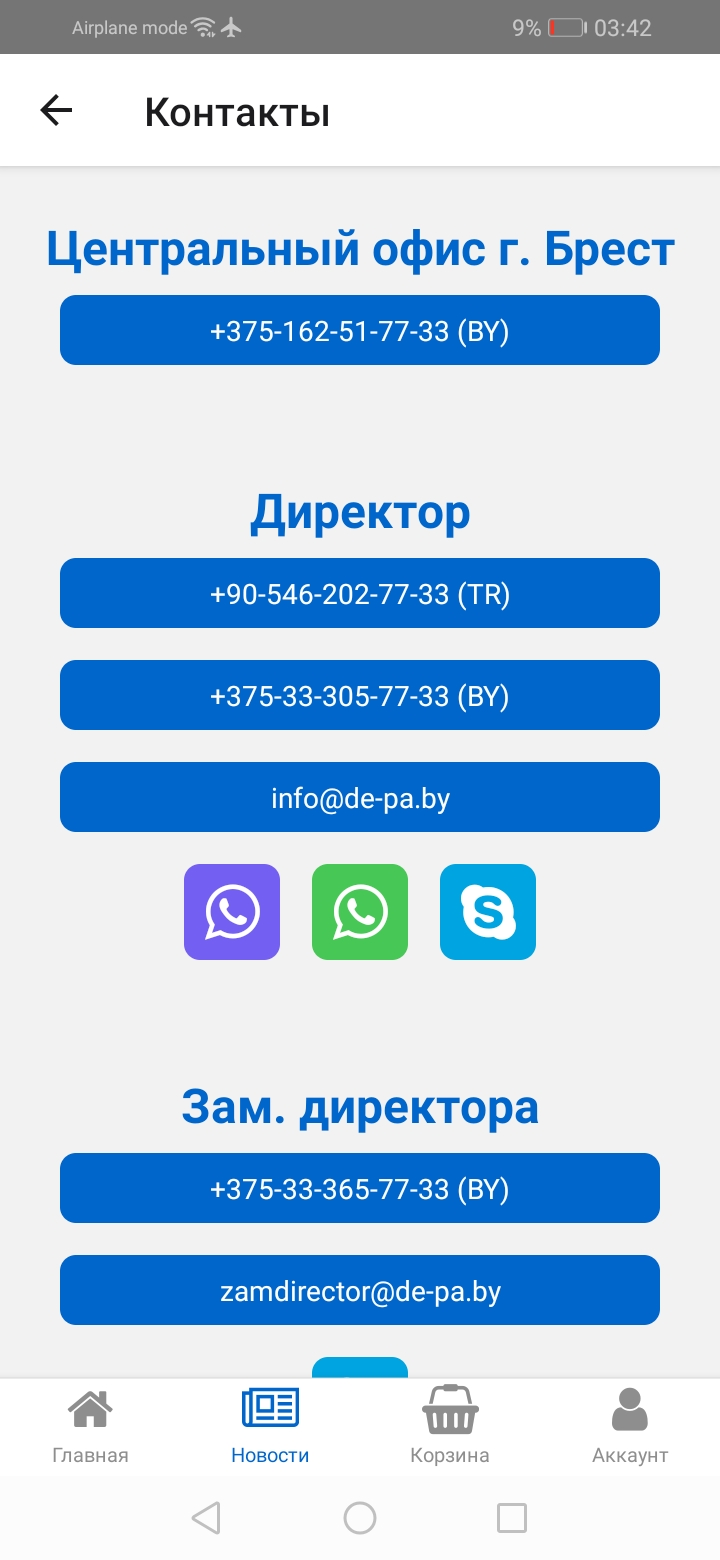
\includegraphics[width=.99\linewidth]
        {images/android/article-contacts.jpg}
    \end{minipage}

    \caption{Прайсы, каталоги, сертификаты, контакты}
    \label{fig:android_articles}
\end{figure}

\begin{figure}[!p]\centering
    \begin{minipage}{0.49\textwidth}
        \centering

        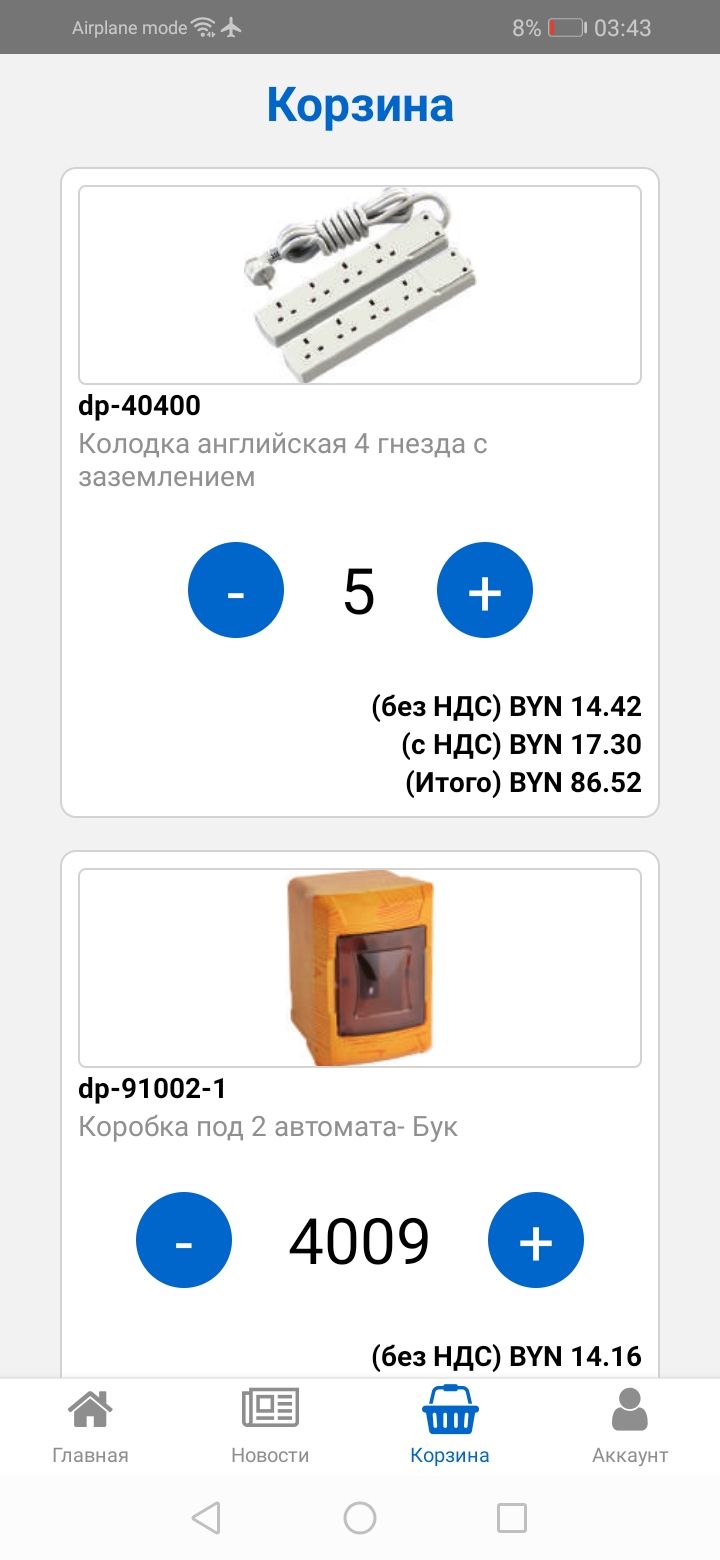
\includegraphics[height=6cm]
        {images/android/basket.jpg}
    \end{minipage}
    \begin{minipage}{0.49\textwidth}
        \centering

        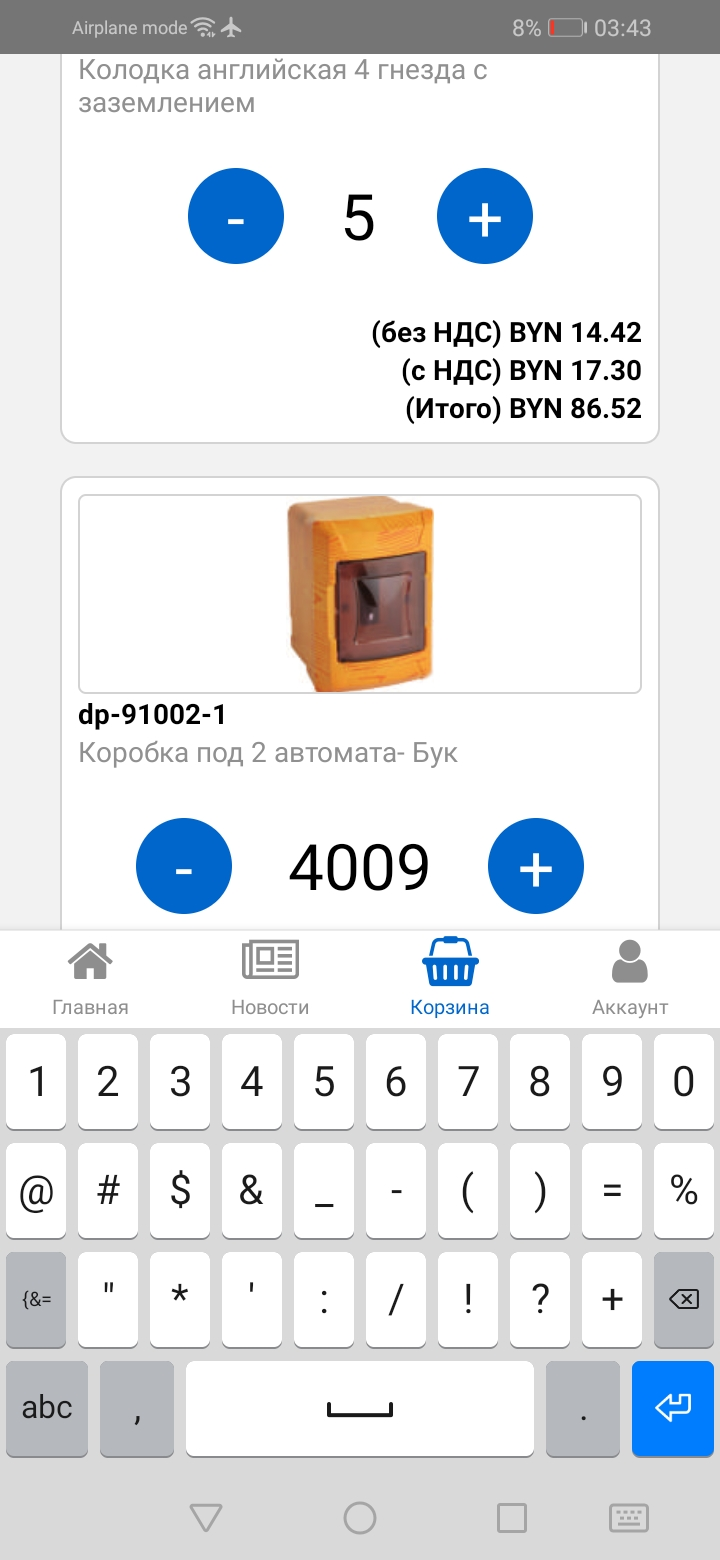
\includegraphics[height=6cm]
        {images/android/basket-change.jpg}
    \end{minipage}

    \caption{Корзина}
    \label{fig:android_basket}
\end{figure}

\begin{figure}[!p]\centering
    \begin{minipage}{0.24\textwidth}
        \centering

        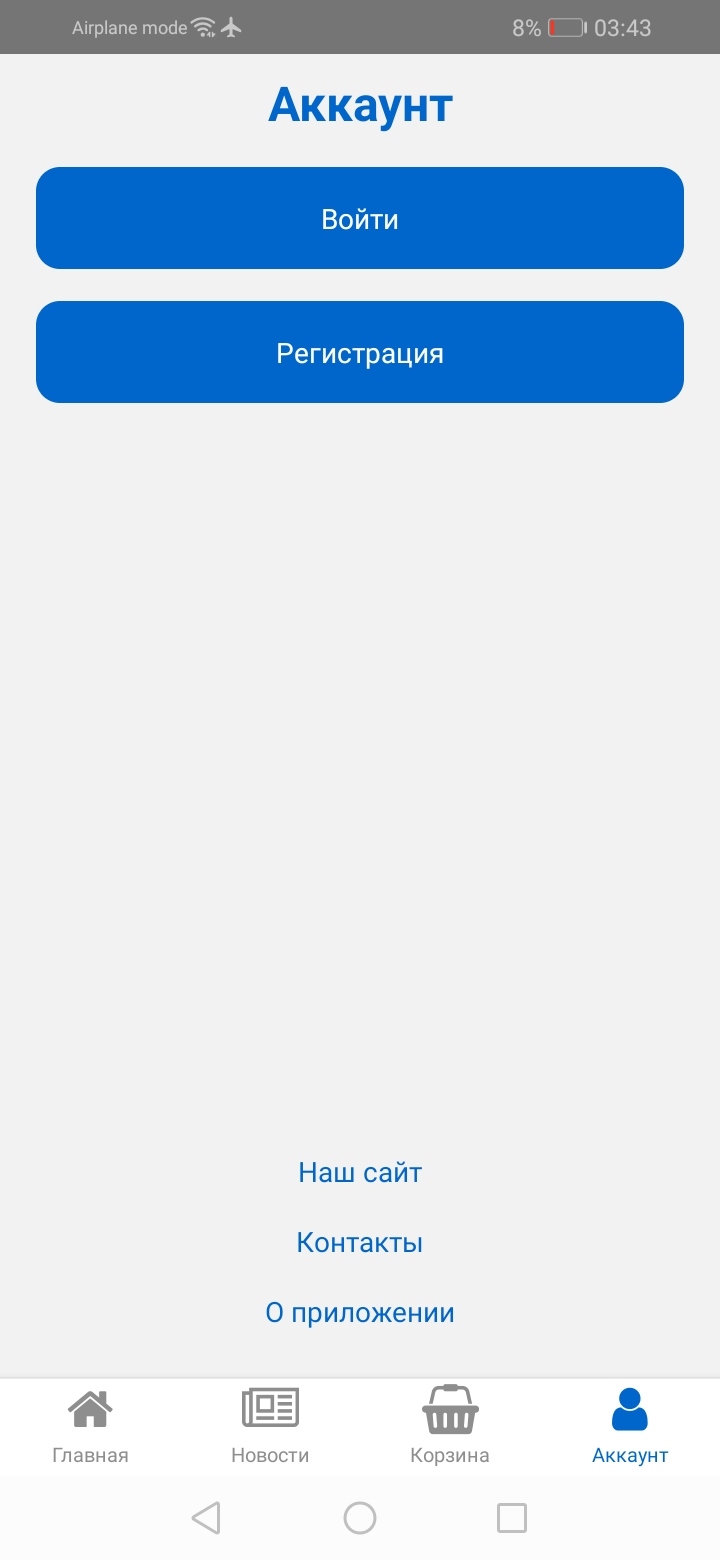
\includegraphics[height=9cm]
        {images/android/account.jpg}
    \end{minipage}
    \begin{minipage}{0.24\textwidth}
        \centering

        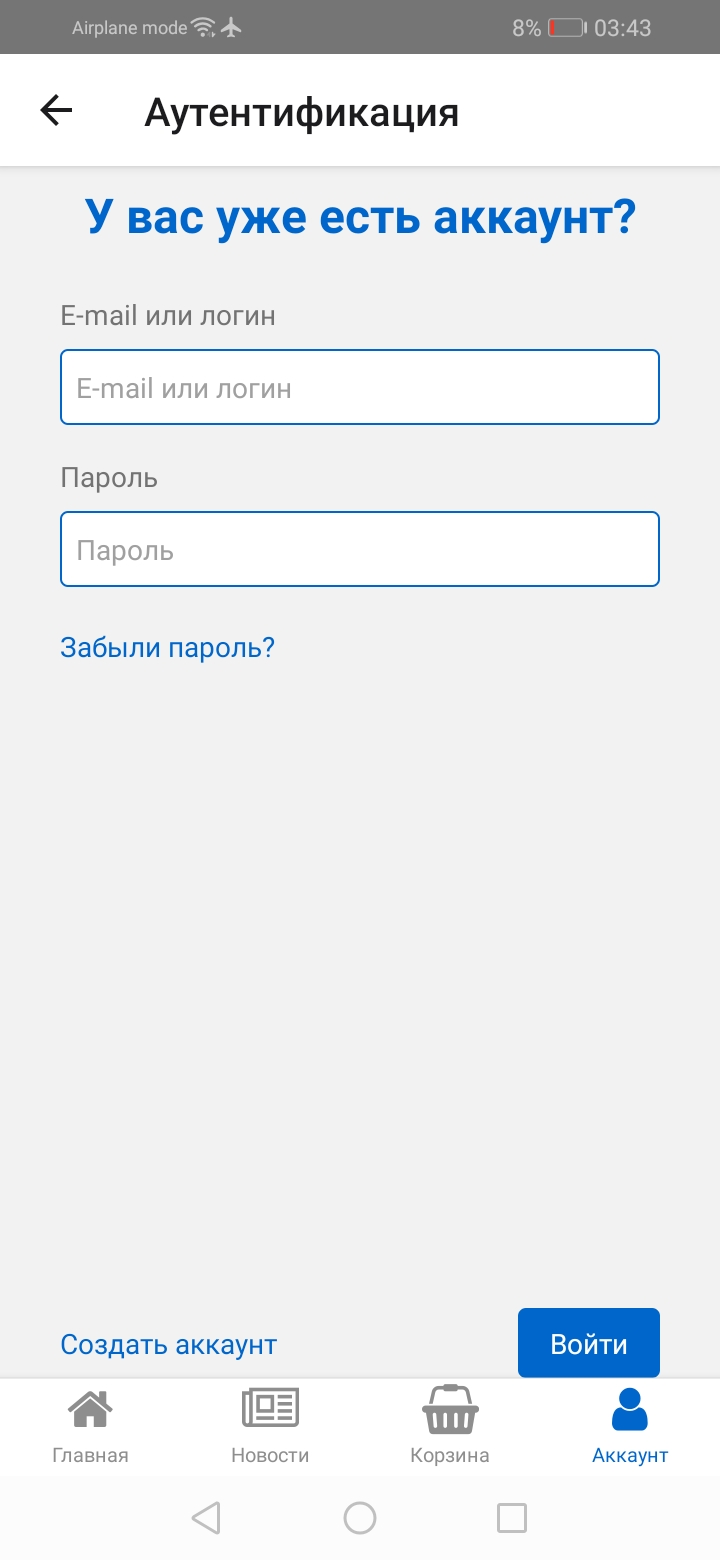
\includegraphics[height=9cm]
        {images/android/account-login.jpg}
    \end{minipage}
    \begin{minipage}{0.24\textwidth}
        \centering

        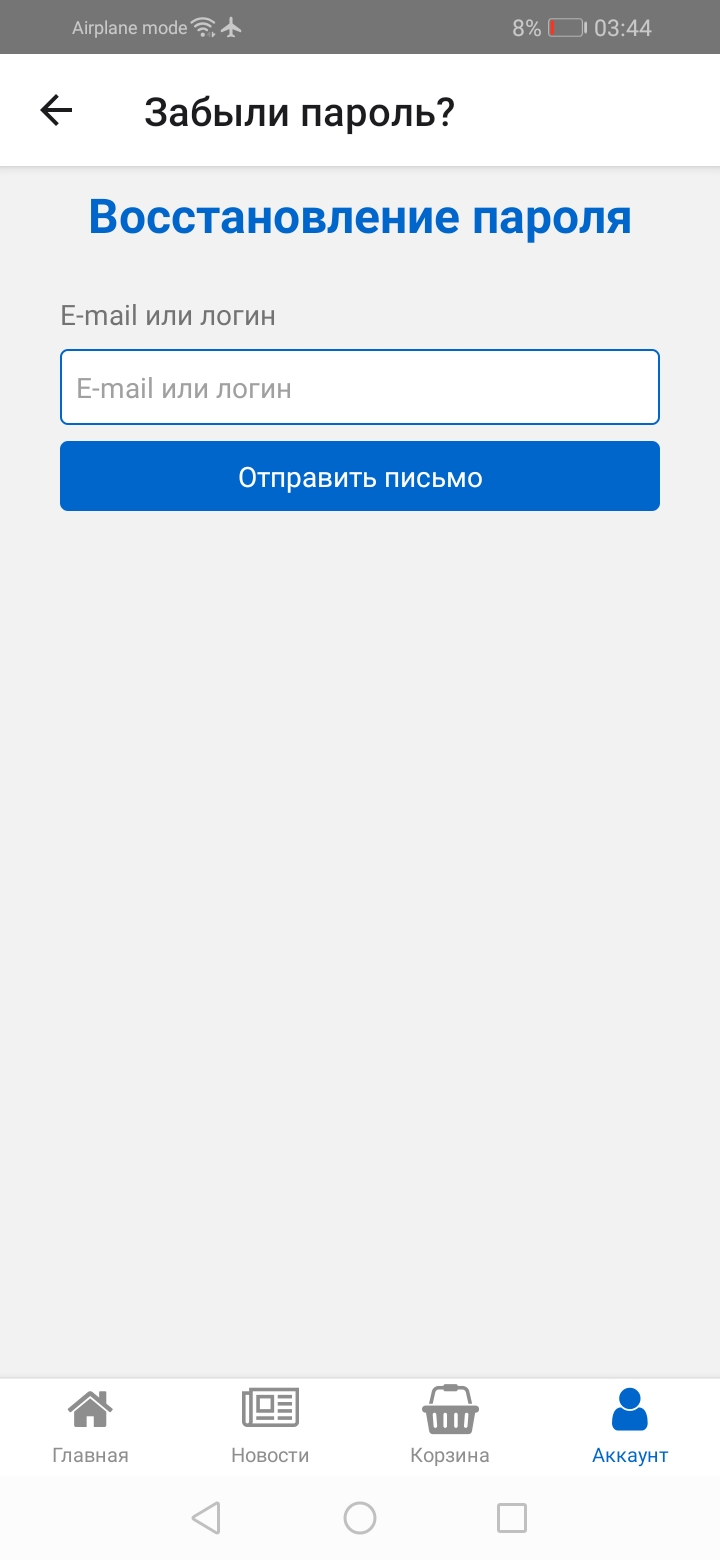
\includegraphics[height=9cm]
        {images/android/account-forget-password.jpg}
    \end{minipage}
    \begin{minipage}{0.24\textwidth}
        \centering

        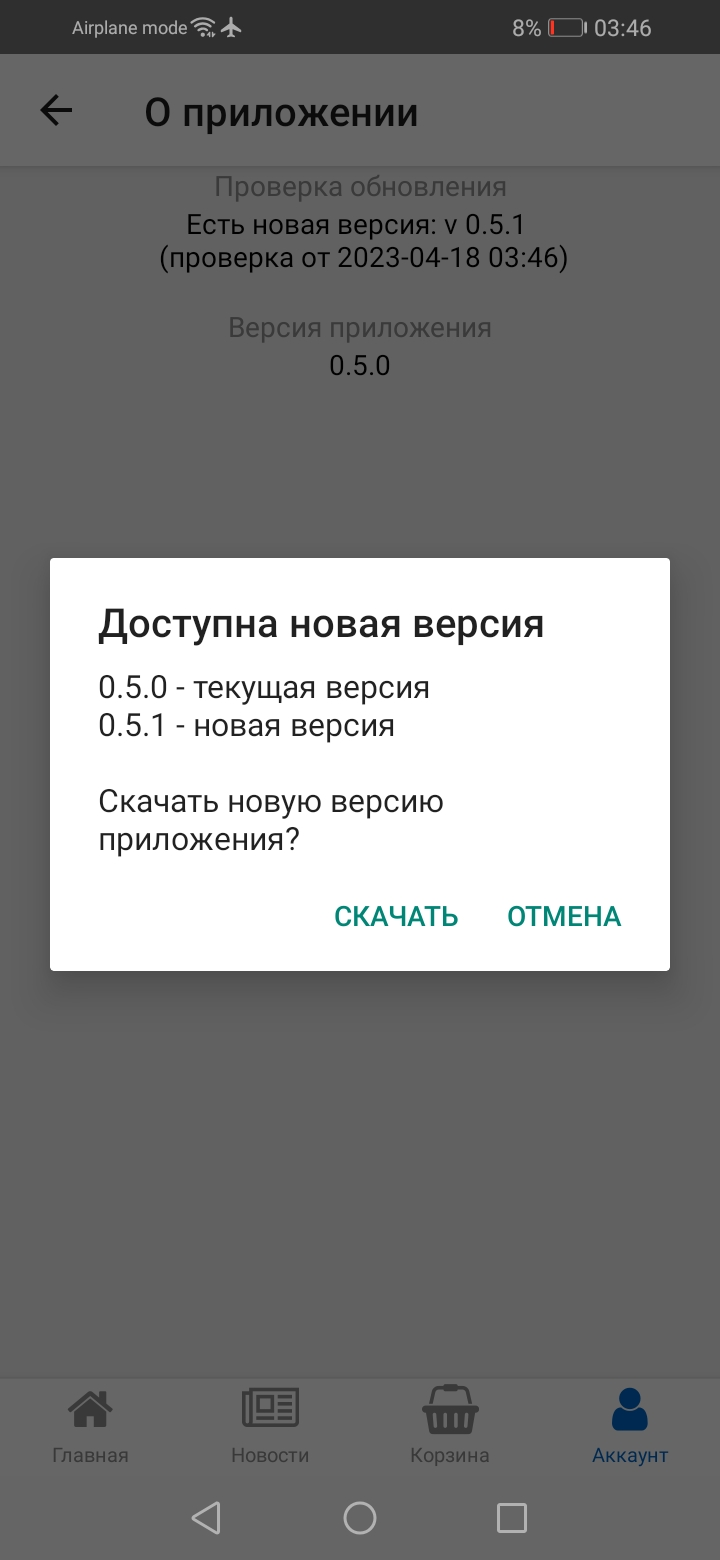
\includegraphics[height=9cm]
        {images/android/account-versions.jpg}
    \end{minipage}

    \caption{Вход в аккаунт, восстановление пароля, проверка новой версии}
    \label{fig:android_login}
\end{figure}

\begin{figure}[!p]\centering
    \begin{minipage}{0.24\textwidth}
        \centering

        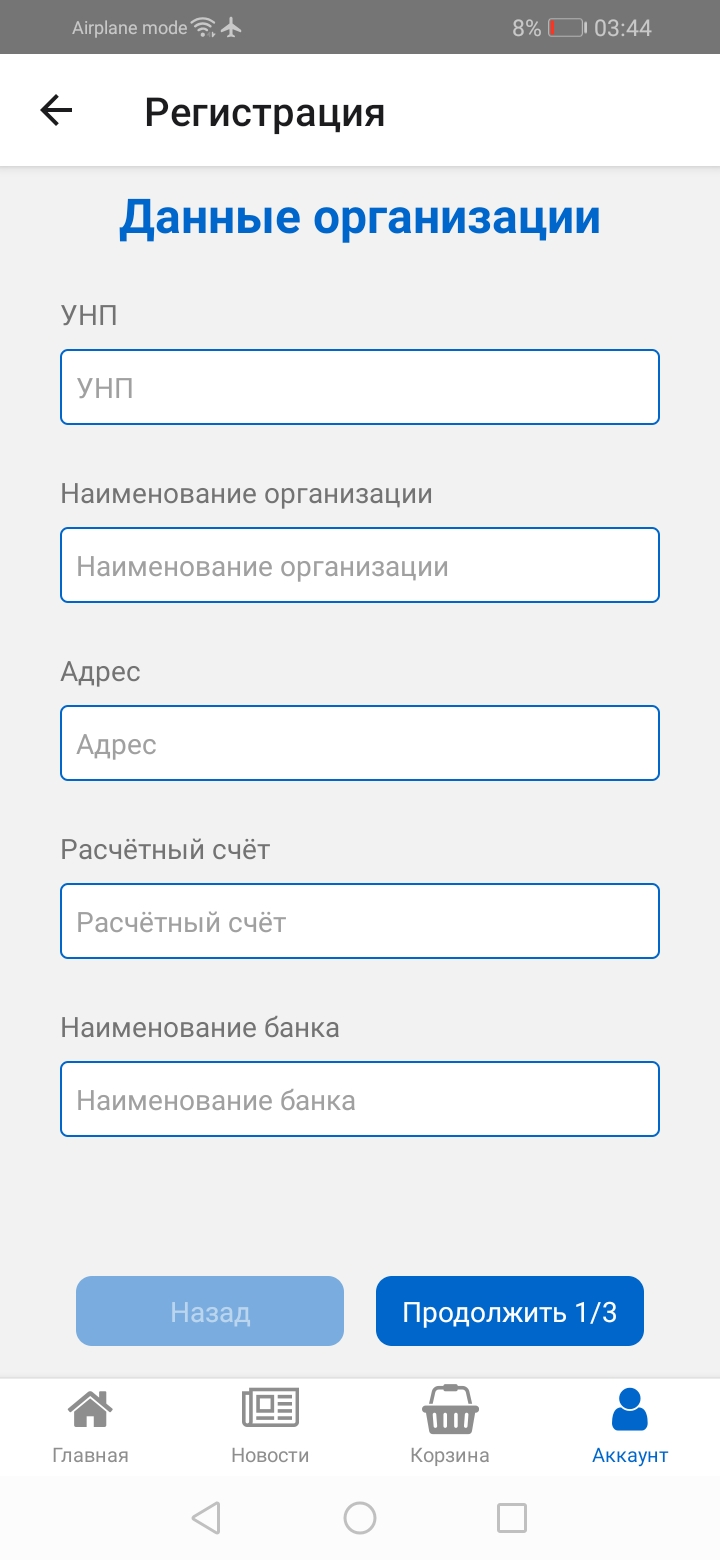
\includegraphics[height=10cm]
        {images/android/account-registration-step1.jpg}
    \end{minipage}
    \begin{minipage}{0.24\textwidth}
        \centering

        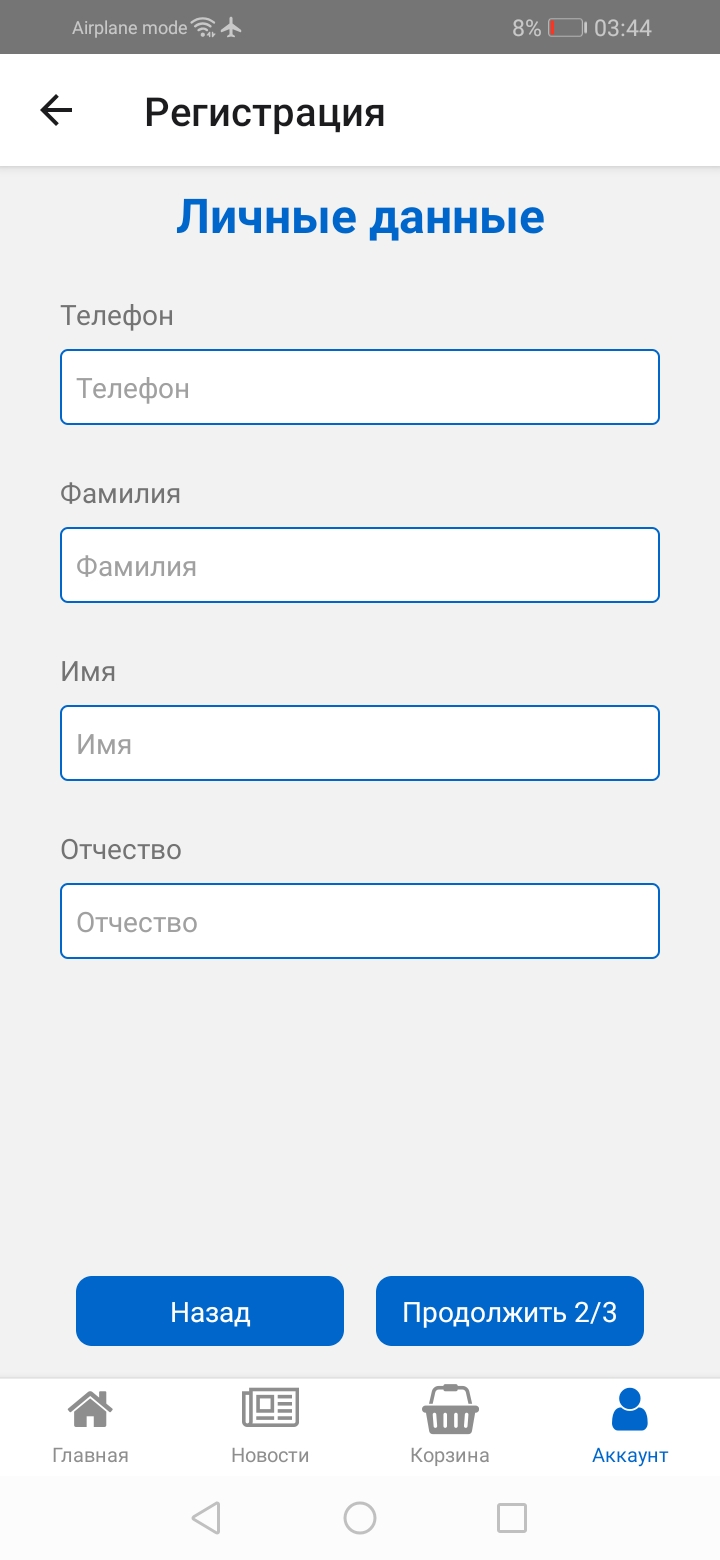
\includegraphics[height=10cm]
        {images/android/account-registration-step2.jpg}
    \end{minipage}
    \begin{minipage}{0.24\textwidth}
        \centering

        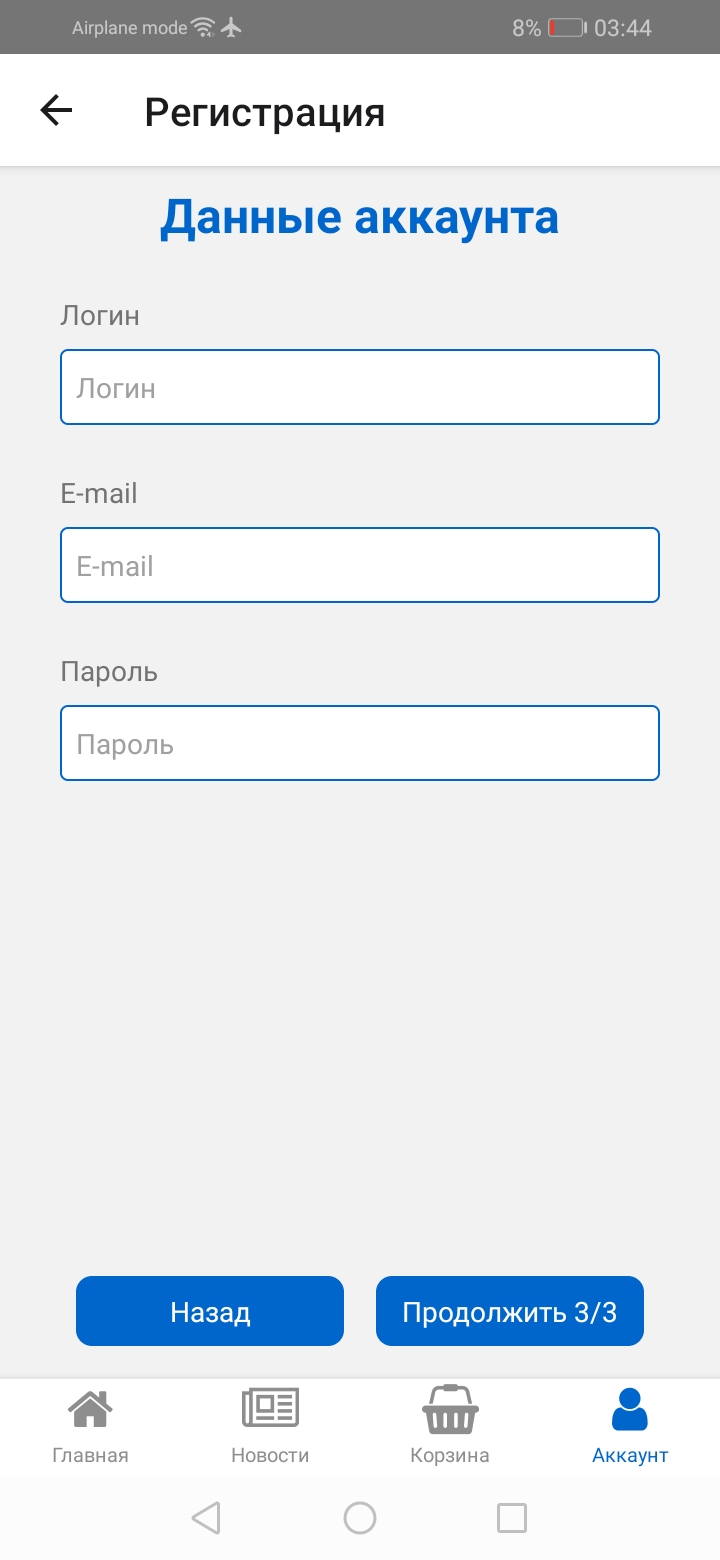
\includegraphics[height=10cm]
        {images/android/account-registration-step3.jpg}
    \end{minipage}
    \begin{minipage}{0.24\textwidth}
        \centering

        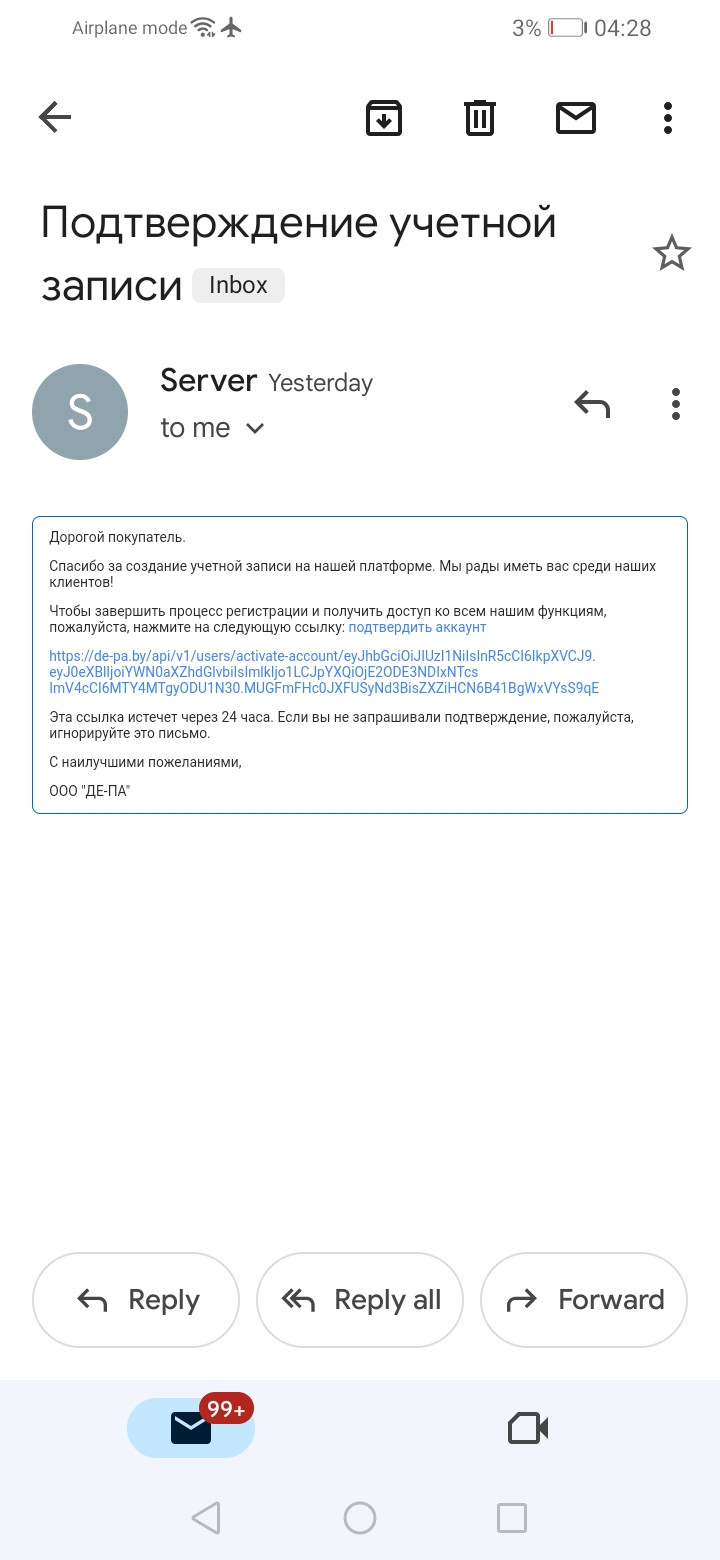
\includegraphics[height=10cm]
        {images/android/account-registration-step4.jpg}
    \end{minipage}

    \caption{Регистрация юридического лица}
    \label{fig:android_registration}
\end{figure}
